% ============================================
% 5 问题2：分类规律与亚类划分
% ============================================
\section{问题2：分类规律与亚类划分}

\subsection{高钾与铅钡玻璃的分类规律}

\subsubsection{数据准备}

以未风化样品为训练集（高钾 12、铅钡 13），风化样品为测试集（高钾 6、铅钡 36）。训练集无风化干扰，可反映原始配方的分类特征。

\subsubsection{研究方法}

\begin{enumerate}[label=(\arabic*)]
    \item \textbf{单氧化物判别力评估}：Mann-Whitney U 检验 $+$ Cohen's $d$ 效应量 $+$ ROC-AUC
    \item \textbf{决策树分类}：CART 算法，$\text{max\_depth} = 3$，5 折交叉验证
    \item \textbf{线性判别分析（LDA）}：多变量线性判别，5 折交叉验证
\end{enumerate}

\subsubsection{结果分析}

\textbf{单氧化物判别力}：

\begin{table}[H]
    \centering
    \caption{单氧化物对玻璃类型的判别力}
    \label{tab:oxide_discrimination}
    \begin{tabular}{l c c c c}
        \toprule
        \textbf{氧化物} & \textbf{AUC} & \textbf{Cohen's $d$} & \textbf{$p$ 值} & \textbf{判别力} \\
        \midrule
        PbO & \textbf{1.000} & 3.74 & $< 0.001$ & 完美 \\
        BaO & \textbf{1.000} & 2.08 & $< 0.001$ & 完美 \\
        SrO & 0.712 & 1.18 & 0.065 & 一般 \\
        $\text{K}_2\text{O}$ & 0.067 & 3.40 & $< 0.001$ & 反向完美 \\
        \bottomrule
    \end{tabular}
\end{table}

PbO 和 BaO 均达到 $\text{AUC} = 1.0$（完美分离）。$\text{K}_2\text{O}$ 虽然效应量极大，但高钾玻璃 $\text{K}_2\text{O}$ 高、铅钡玻璃 $\text{K}_2\text{O}$ 低——方向与 PbO/BaO 相反，$\text{AUC} = 0.067$ 是因为高值指向高钾类（标记为 0）而非铅钡（标记为 1）。

\textbf{决策树分类规则}：

\begin{verbatim}
    BaO <= 3.14%  =>  高钾玻璃
    BaO > 3.14%   =>  铅钡玻璃
\end{verbatim}

仅需一条规则即可完美分类训练数据。

\textbf{模型性能对比}：

\begin{table}[H]
    \centering
    \caption{分类模型性能对比}
    \label{tab:classifier_performance}
    \begin{tabular}{l c c}
        \toprule
        \textbf{模型} & \textbf{训练集 CV 准确率} & \textbf{风化测试集准确率} \\
        \midrule
        决策树 & 92.0\% & \textbf{90.5\%} \\
        LDA & 76.0\% & 61.9\% \\
        \bottomrule
    \end{tabular}
\end{table}

决策树基于 BaO 单特征分类，对风化高度鲁棒——BaO 在风化过程中相对稳定，不易流失。LDA 过度依赖多种次要特征（SrO、$\text{SnO}_2$、MgO），在训练集上过拟合，泛化能力差。

\subsubsection{结论}

\textbf{BaO $> 3.14\%$ 是铅钡玻璃的可靠判别标志}。该规则简洁、可解释性强、对风化干扰不敏感，准确率 $> 90\%$。

\begin{figure}[H]
    \centering
    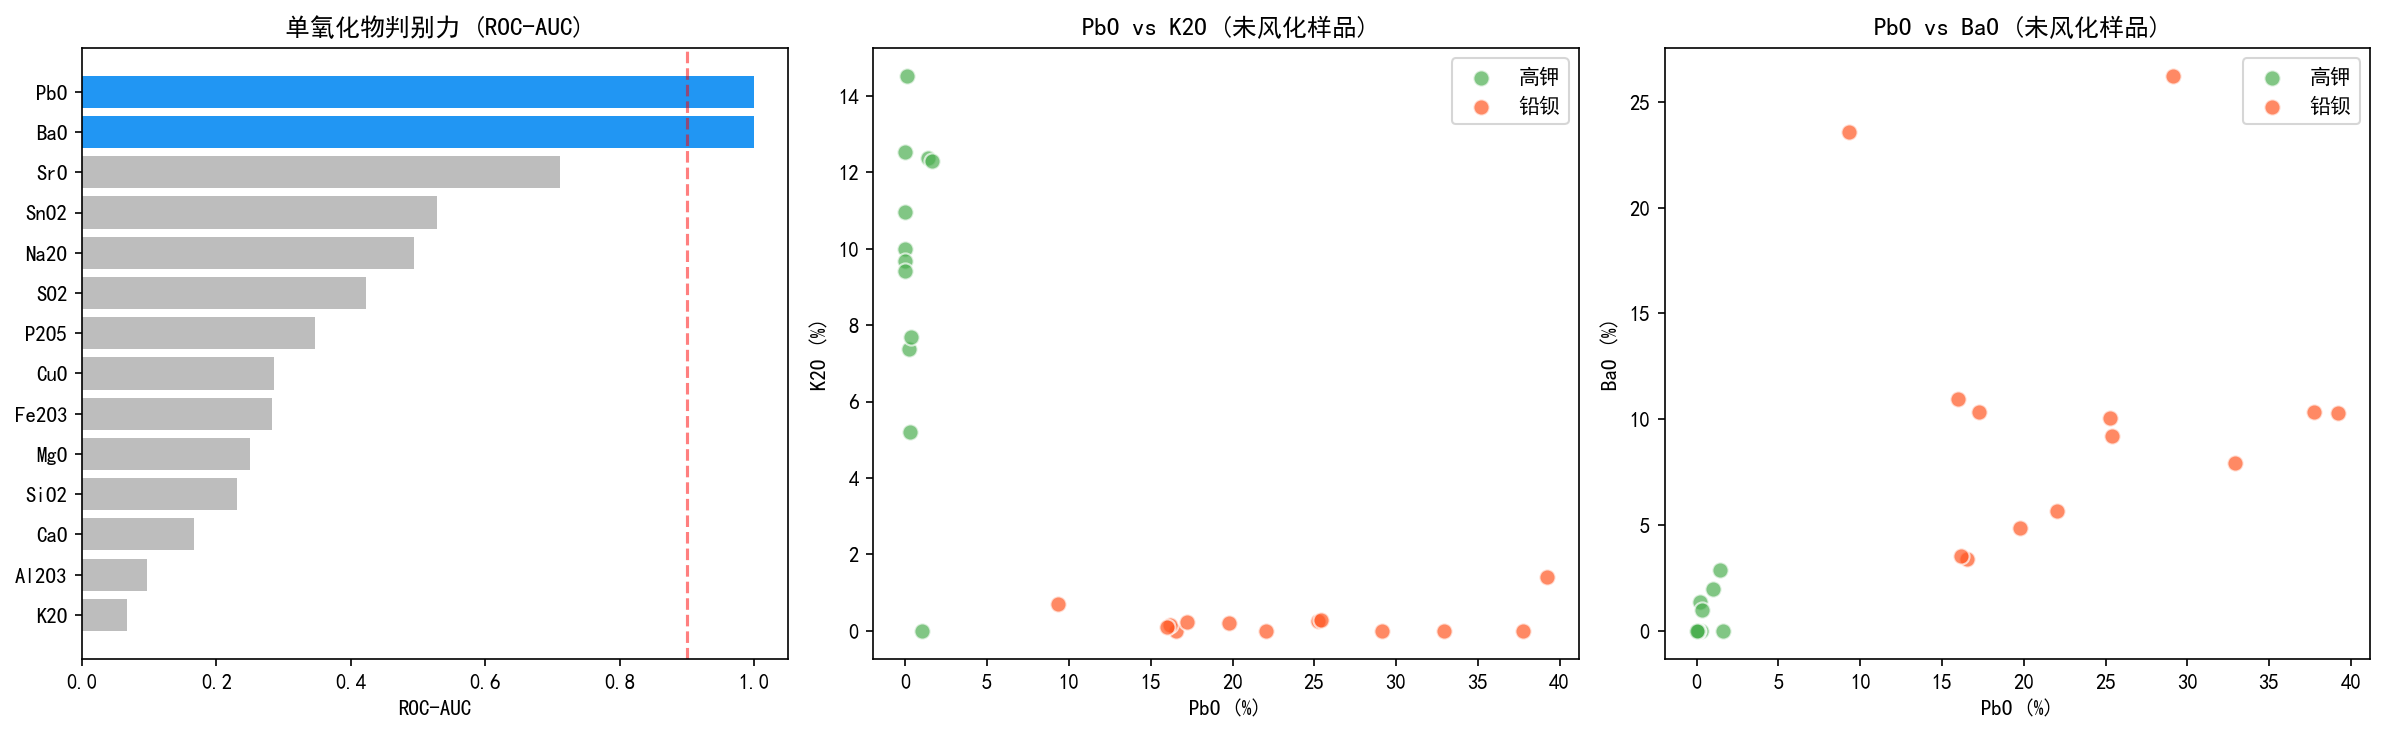
\includegraphics[width=0.85\textwidth]{../analysis/fig2a_discrimination.png}
    \caption{分类判别力图（AUC 横棒 $+$ PbO-$\text{K}_2\text{O}$ 散点 $+$ PbO-BaO 散点）}
    \label{fig:discrimination}
\end{figure}

\begin{figure}[H]
    \centering
    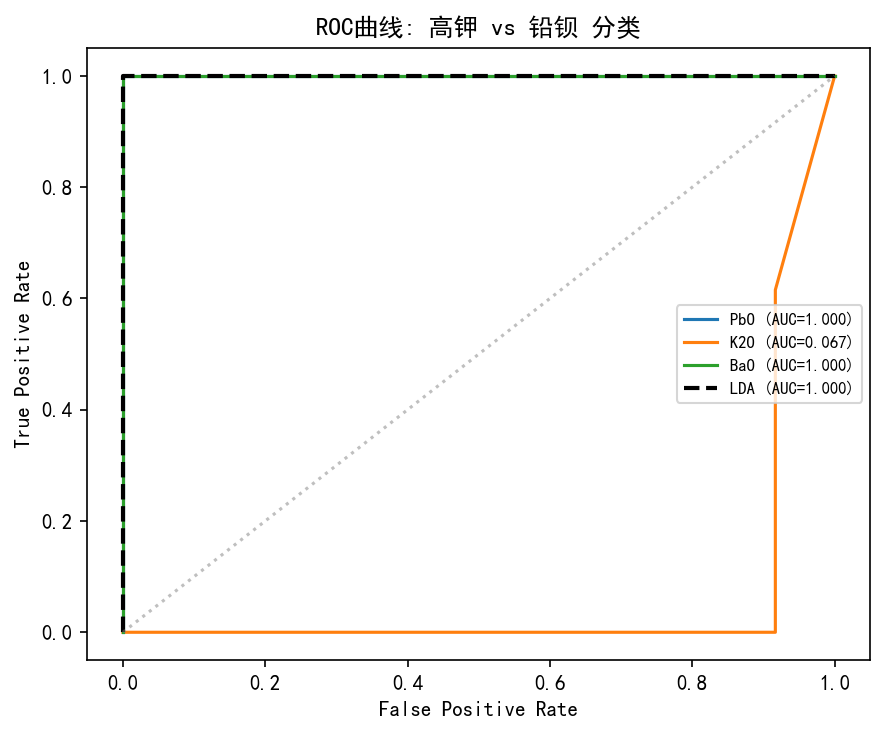
\includegraphics[width=0.85\textwidth]{../analysis/fig2a_roc.png}
    \caption{ROC 曲线对比}
    \label{fig:roc}
\end{figure}

\subsection{亚类划分}

\subsubsection{研究方法}

对高钾玻璃（18 个采样点）和铅钡玻璃（49 个采样点）分别进行亚类分析：

\begin{enumerate}[label=(\arabic*)]
    \item \textbf{数据预处理}：$Z$-score 标准化，使各氧化物具有相同尺度
    \item \textbf{PCA 降维}：保留累计方差贡献率 $\geq 85\%$ 的主成分
    \item \textbf{$K$-means 聚类}：以肘部法则和轮廓系数确定最佳聚类数 $k$
    \item \textbf{敏感性分析}：
    \begin{itemize}
        \item Bootstrap 重采样（100 次）$\rightarrow$ 调整 Rand 指数（ARI）
        \item 噪声扰动（$\pm 5\%$ 高斯噪声）$\rightarrow$ ARI
    \end{itemize}
\end{enumerate}

\subsubsection{高钾玻璃亚类（$k = 4$）}

\begin{itemize}
    \item 轮廓系数：\textbf{0.514}
    \item Bootstrap ARI：0.833（中等敏感）
    \item 扰动 ARI：\textbf{1.000}（高度鲁棒）
\end{itemize}

\begin{table}[H]
    \centering
    \caption{高钾玻璃 4 个亚类的化学成分特征}
    \label{tab:hk_subclass}
    \begin{tabular}{c c c c c c c}
        \toprule
        \textbf{亚类} & \textbf{样本量} & \textbf{$\text{SiO}_2$} & \textbf{$\text{K}_2\text{O}$} & \textbf{CaO} & \textbf{$\text{Al}_2\text{O}_3$} & \textbf{特征解读} \\
        \midrule
        A & 3 & 65.6\% & 10.2\% & 6.9\% & 6.0\% & 经典高钾配方 \\
        B & 8 & \textbf{91.3\%} & 2.2\% & —— & 2.3\% & 风化高钾（淋溶残留） \\
        C & 4 & 66.5\% & 6.9\% & 4.0\% & 8.2\% & 铁铝偏高型 \\
        D & 3 & 62.2\% & 13.1\% & 8.4\% & 7.2\% & 钠钙富集型 \\
        \bottomrule
    \end{tabular}
\end{table}

亚类 B 本质为风化高钾玻璃，其余 3 个亚类反映原始配方的化学多样性，但各亚类仅 3$\sim$4 个样本，统计说服力有限。

\subsubsection{铅钡玻璃亚类（$k = 3$）}

\begin{itemize}
    \item 轮廓系数：\textbf{0.264}
    \item Bootstrap ARI：0.635（中等敏感）
    \item 扰动 ARI：\textbf{0.959}（高度鲁棒）
\end{itemize}

\begin{table}[H]
    \centering
    \caption{铅钡玻璃 3 个亚类的化学成分特征}
    \label{tab:pb_subclass}
    \begin{tabular}{c c c c c c c c}
        \toprule
        \textbf{亚类} & \textbf{样本量} & \textbf{$\text{SiO}_2$} & \textbf{PbO} & \textbf{BaO} & \textbf{$\text{P}_2\text{O}_5$} & \textbf{CuO} & \textbf{特征解读} \\
        \midrule
        A & 18 & 25.3\% & \textbf{46.8\%} & 7.1\% & 6.3\% & —— & 严重风化/高铅型 \\
        B & 5 & 16.0\% & 29.9\% & \textbf{31.2\%} & 4.1\% & \textbf{7.2\%} & 高钡高铜型 \\
        C & 26 & \textbf{52.7\%} & 24.7\% & 8.9\% & 1.0\% & 1.1\% & 轻度风化/硅质型 \\
        \bottomrule
    \end{tabular}
\end{table}

铅钡玻璃的 3 个亚类本质上是\textbf{风化程度的连续谱}：C $\rightarrow$ A $\rightarrow$ B 对应 $\text{SiO}_2$ 递减（53\% $\rightarrow$ 25\% $\rightarrow$ 16\%）、PbO 递增（25\% $\rightarrow$ 47\% $\rightarrow$ 30\%）、$\text{P}_2\text{O}_5$ 和 $\text{SO}_2$ 递增。亚类 B 对应 08、26、54 的严重风化点，CuO 极高（7.2\% vs 1$\sim$1.5\%），代表极端风化产物。

\subsubsection{敏感性分析结论}

两类亚类对 $\pm 5\%$ 测量噪声高度鲁棒（ARI $> 0.95$），但对重采样敏感度中等（ARI $0.64\sim0.83$），这是由于样本量有限、个别样品的归属在重采样时可能发生变化。

\begin{figure}[H]
    \centering
    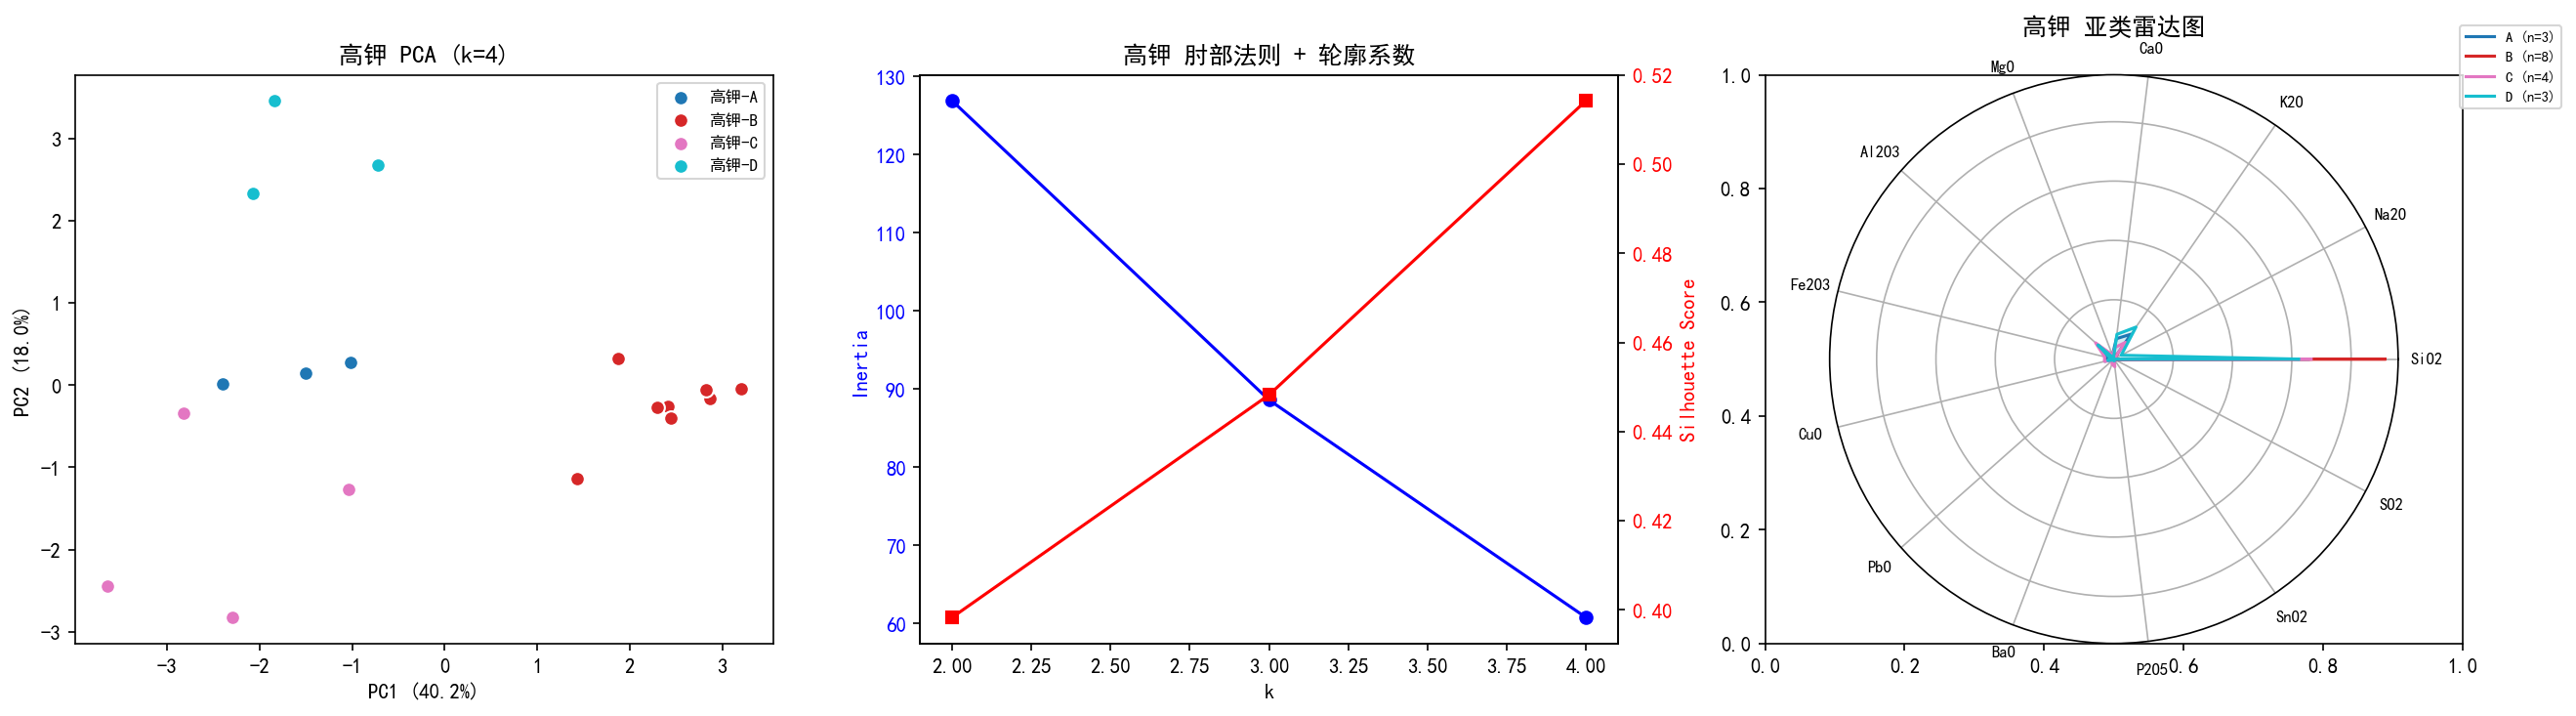
\includegraphics[width=0.85\textwidth]{../analysis/fig2b_高钾_subclass.png}
    \caption{高钾亚类聚类结果（PCA 散点 $+$ 肘部法则 $+$ 雷达图）}
    \label{fig:hk_subclass_fig}
\end{figure}

\begin{figure}[H]
    \centering
    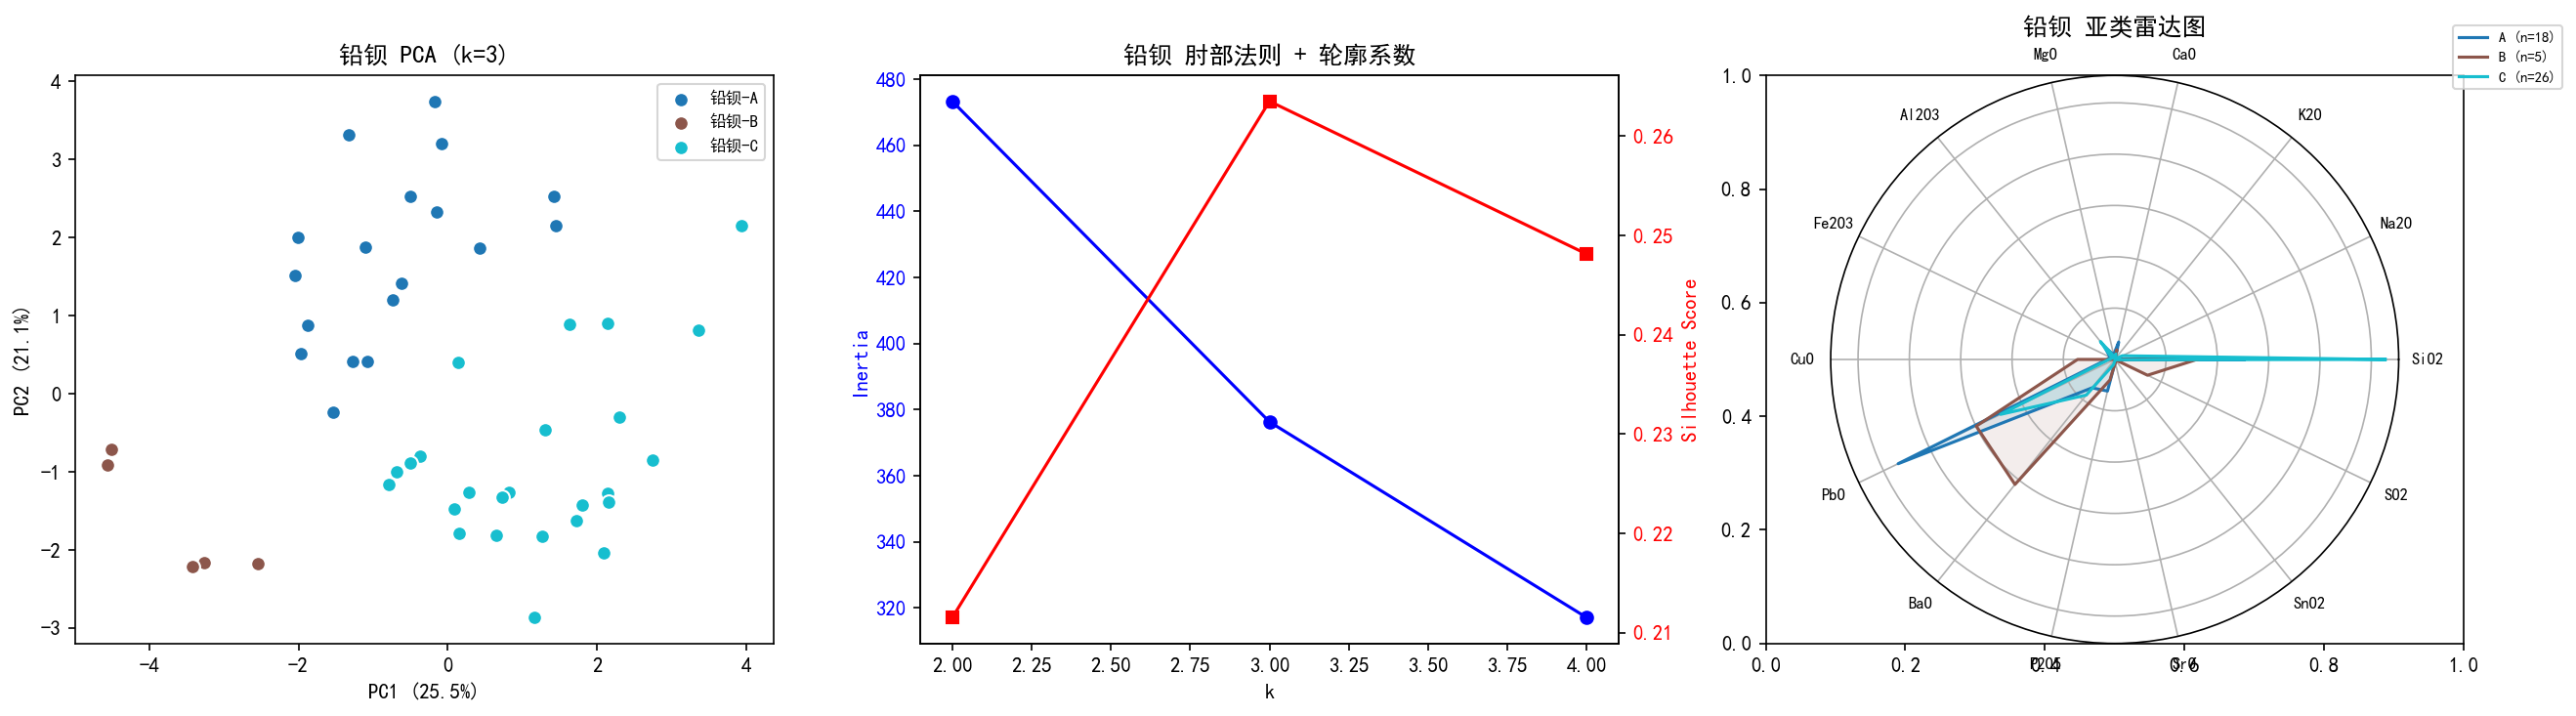
\includegraphics[width=0.85\textwidth]{../analysis/fig2b_铅钡_subclass.png}
    \caption{铅钡亚类聚类结果（PCA 散点 $+$ 肘部法则 $+$ 雷达图）}
    \label{fig:pb_subclass_fig}
\end{figure}
